\documentclass[10pt]{article}
\usepackage{float}
\RequirePackage{eso-pic}
\usepackage{caption}
\captionsetup[table]{labelformat=empty}



\usepackage{geometry}
\geometry{
a4paper,
left=11mm,
right=14mm,
top=37mm,
bottom=14mm,
}



\usepackage{colortbl}
\usepackage{fontspec}
\setmainfont[Ligatures=TeX]{Calibri}



\newcommand\BackgroundPic{%
\put(0,0){%
\parbox[b][\paperheight]{\paperwidth}{%
\vfill
\centering
\includegraphics{MBIE_generic_background.pdf}%
\vfill
}}}



\begin{document}
\thispagestyle{empty}
\AddToShipoutPicture{\BackgroundPic}
\section*{Key Export Statistics\footnotemark - Capsicums\footnotemark }
Published on April 11, 2016. \par
\small{\noindent{\textit{Monthly data from January 2000 to November 2015.}}}
\begin{table}[ht]
\centering
{\scriptsize
\begin{tabular}[t]{p{1.8cm}>{\hfill}p{1.4cm}>{\hfill}p{1.4cm}>{\hfill}p{1.6cm}>{\hfill}p{1.9cm}>{\hfill}p{2cm}>{\hfill}p{1.9cm}>{\hfill}p{1.5cm}}
 \textbf{Country} & \textbf{Yearly Qty} & \textbf{Yearly Value} & \textbf{Yearly Price} & \textbf{3Year CAGR(Qty)} & \textbf{3Year CAGR(Value)} & \textbf{3Year CAGR(Price)} & \textbf{Price Elasticity} \\
\hline
Japan & 5,281 & 19.6 & \$3.7 & -5\% & -10.4\% & -5.7\% & 0.9 \\  
Australia & 1,720 & 7.3 & \$4.3 & 1.2\% & -8.1\% & -9.2\% & -0.1 \\  
Fiji & 67 & 0.3 & \$4.7 & 8.2\% & 4.9\% & -3\% & -2.7 \\  
French Polynesia & 39 & 0.2 & \$5.7 & 11.2\% & 8.4\% & -2.5\% & -4.5 \\  
New Caledonia & 42 & 0.2 & \$5.2 & 4.4\% & -1\% & -5.1\% & -0.9 \\  
Canada & 36 & 0.2 & \$4.4 & 19.5\% & -6.2\% & -21.5\% & -0.9 \\  
Other & 28 & 0.2 & \$6.7 & -84.8\% & -82.9\% & 12.3\% & -6.9 \\  
Total & 7,213 & 28.0 & \$3.9 & 5.4\% & 0.9\% & -4.2\% & -1.3 \\  
\hline
\end{tabular}
}
\caption{\scriptsize Top 6 Capsicums Markets for year ending November - 2015: Quantity('000 kg) Value(NZ\$Mill), Price and their last 3-Year Growth Rates}
\end{table}


\vspace{-0.7cm}



   \begin{figure}[H]
   \centering
    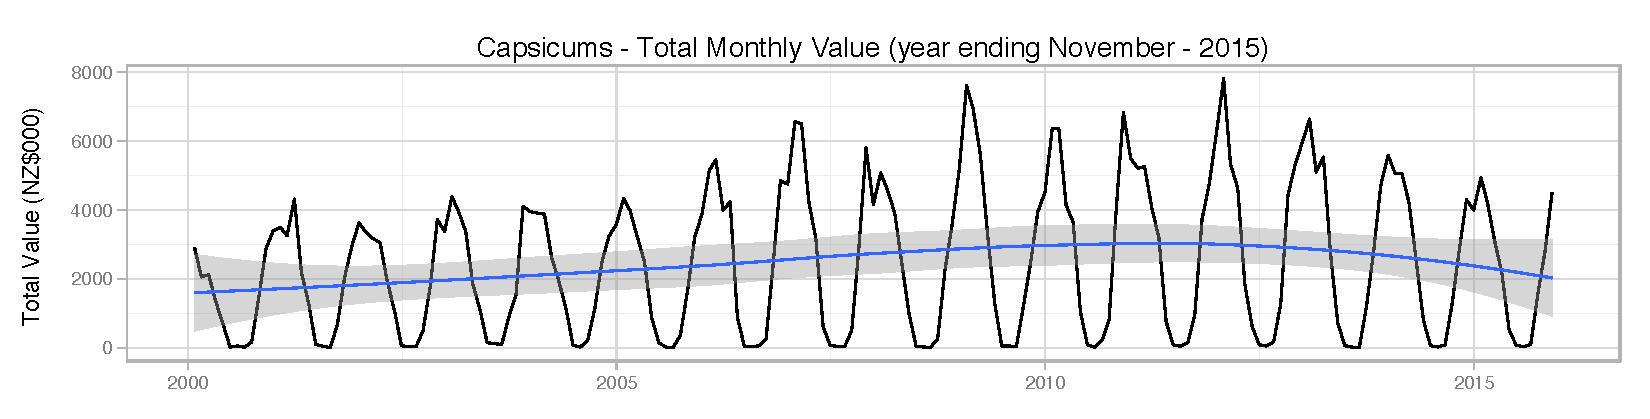
\includegraphics[scale=0.53]{../graphs/monthly_value/capsicums_monthly_value.pdf} \
    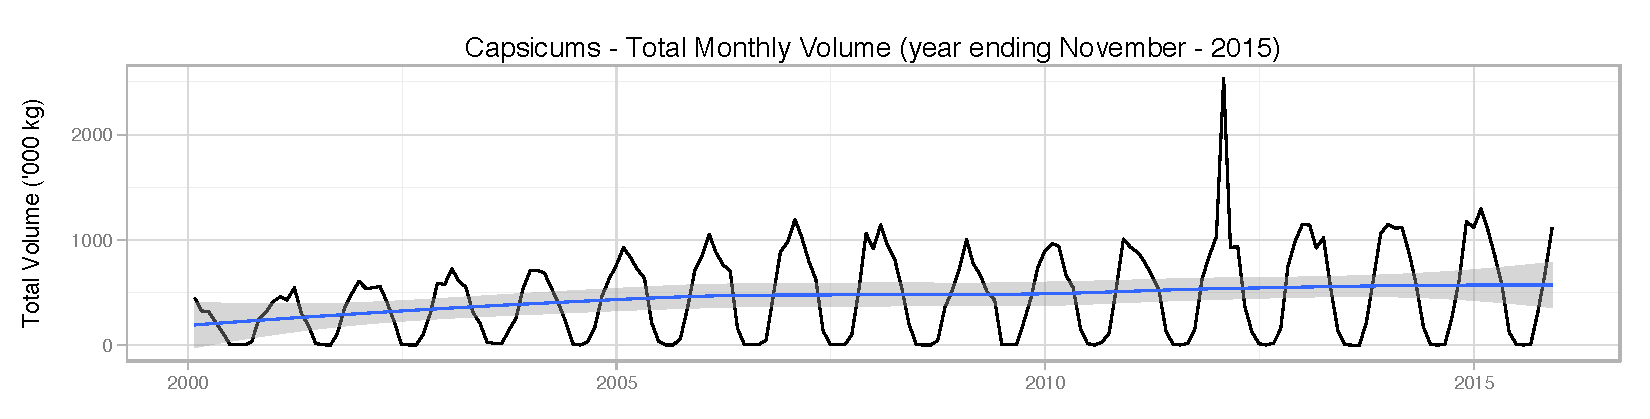
\includegraphics[scale=0.53]{../graphs/monthly_volume/capsicums_monthly_volume.pdf} \
    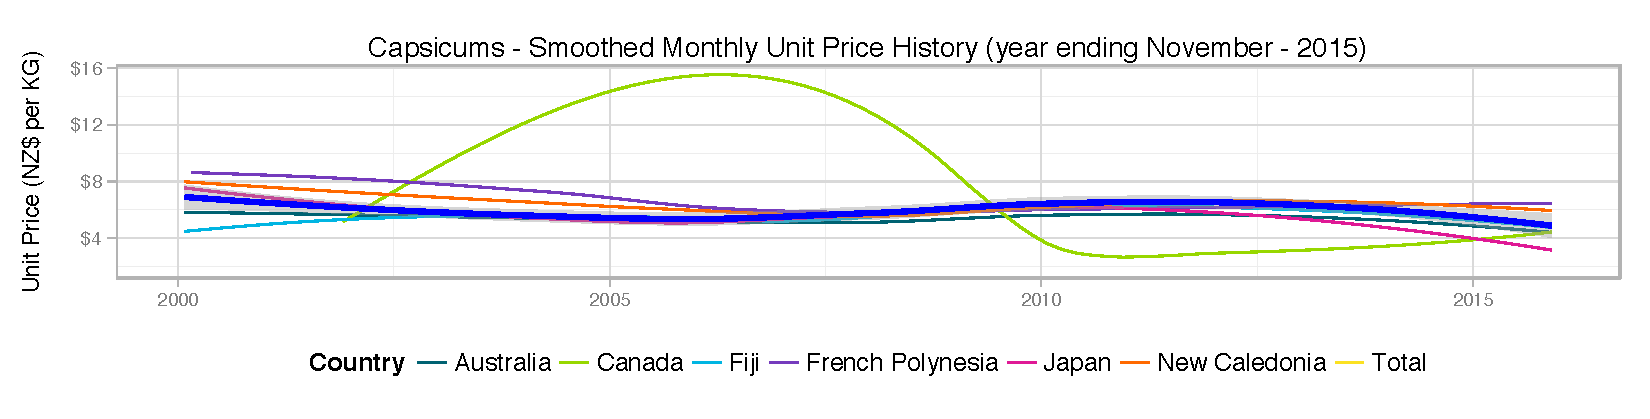
\includegraphics[scale=0.53]{../graphs/smoothed_price/capsicums_smoothed_price.pdf} \
    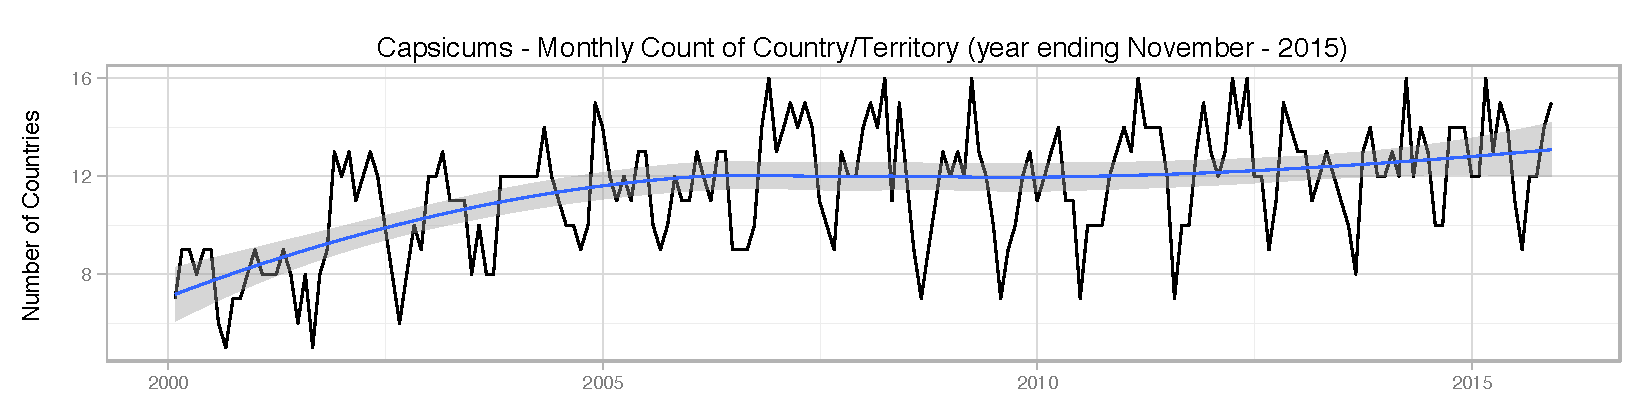
\includegraphics[scale=0.53]{../graphs/monthly_number_countries/capsicums_monthly_count.pdf} \
    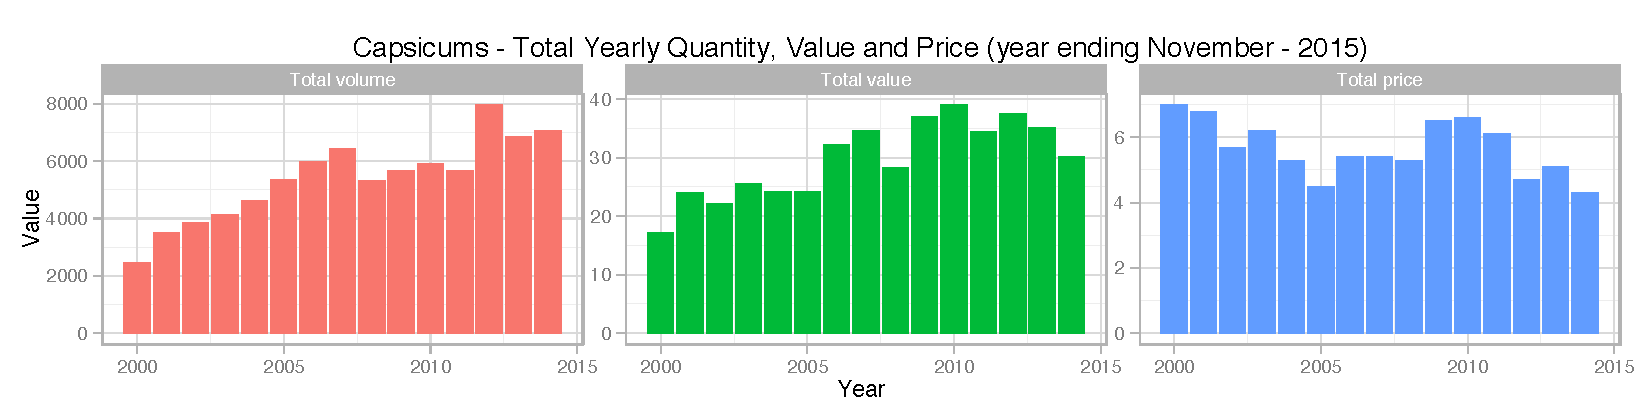
\includegraphics[scale=0.53]{../graphs/yearly_summary/capsicums_yearly_summary.pdf} \
   \end{figure}



\footnotetext[1]{Source: Statistics New Zealand - Overseas Merchandise Trade}
\footnotetext[2]{Harmonised System Codes for Capsicums starting with: 070960.}
\end{document}
